\documentclass{article}
\usepackage{graphicx}
\usepackage{tikz}
\usepackage{comment}
\usepackage{geometry}
\geometry{a4paper, margin=1in}

\title{Tallahassee Crime Map}
\author{Munawar Ali, Çağatay Ayhan, Ece Karaçam, Abdullah Malik, and Mao Nishino}
\date{\today}

\begin{document}

\maketitle

\begin{abstract}
    This document details the development of a generative AI tool designed to predict crime distribution over geographic maps, aiding city planners in assessing potential crime risks. The approach uses a Generative Adversarial Network (GAN), specifically the pix2pix model, to generate crime heatmaps based on geographic input data.
\end{abstract}

\section{Introduction}

In this project, we aim to analyze geographical crime data in Tallahassee, FL, collected from Tallahassee Police Statistics. Specifically, we will conduct statistical and spatial analyses to identify crime patterns and trends. A key feature of our approach is the utilization of the pix2pix generative model, which allows for the prediction of crime heat maps from both existing and hypothetical geographical maps. This enables urban planners to input their future planning designs into our model to identify potential crime hotspots in advance.

\begin{figure}[!htbp]
    \centering
    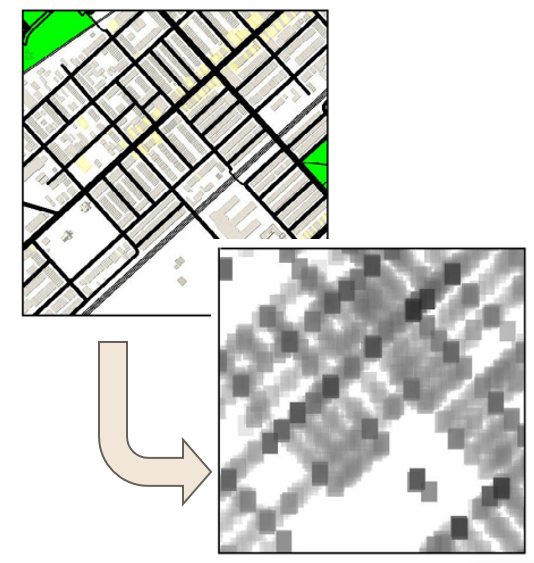
\includegraphics[width=0.5\textwidth]{Figures/Intro Figure.png}
    \caption{Geographical Map to Crime Map (Adapted from He, Zheng 2021)}
\end{figure}

\section{Data Collection and Processing}

Data was collected from the Tallahassee Police Statistics homepage. See Figure \ref{fig:tops} for the visual of the homepage. The dataset is tabular, and the columns includes time of crime reports, crime type, location, and geographical coordinates. As TOPS uses ArcGIS for mapping, we use ArcGIS API for Python to extract the data.

\begin{figure}[!htbp]
    \centering
    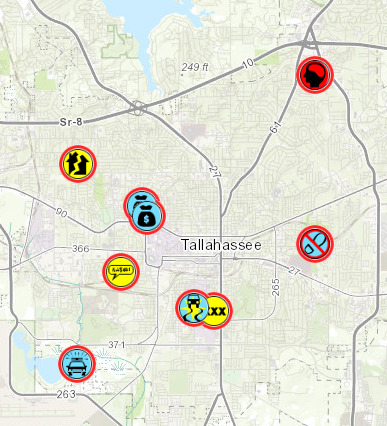
\includegraphics[width=0.5\textwidth]{Figures/TOPS.png}
    \label{fig:tops}
    \caption{Tallahassee Police Statistics Homepage}
\end{figure}

Producing the geographical and the crime heatmap involved using the OSMNx library  Crime data was then superimposed on these maps, with varying degrees of gray dots indicating the frequency of incidents.

\section{Spatial and Temporal Analysis}

\subsection{Categorical Analysis}

A categorical analysis was conducted to identify the frequency of different types of crime reports. The data was visualized using a bar chart that represents each type of crime report in Figure \ref{fig:crime-report}. We observe that many reports are categorized as Community Policing, which is not the direct crime report. To avoid misinterpretation, we will exclude these reports from the analysis.

\begin{figure}[!htbp]
    \centering
    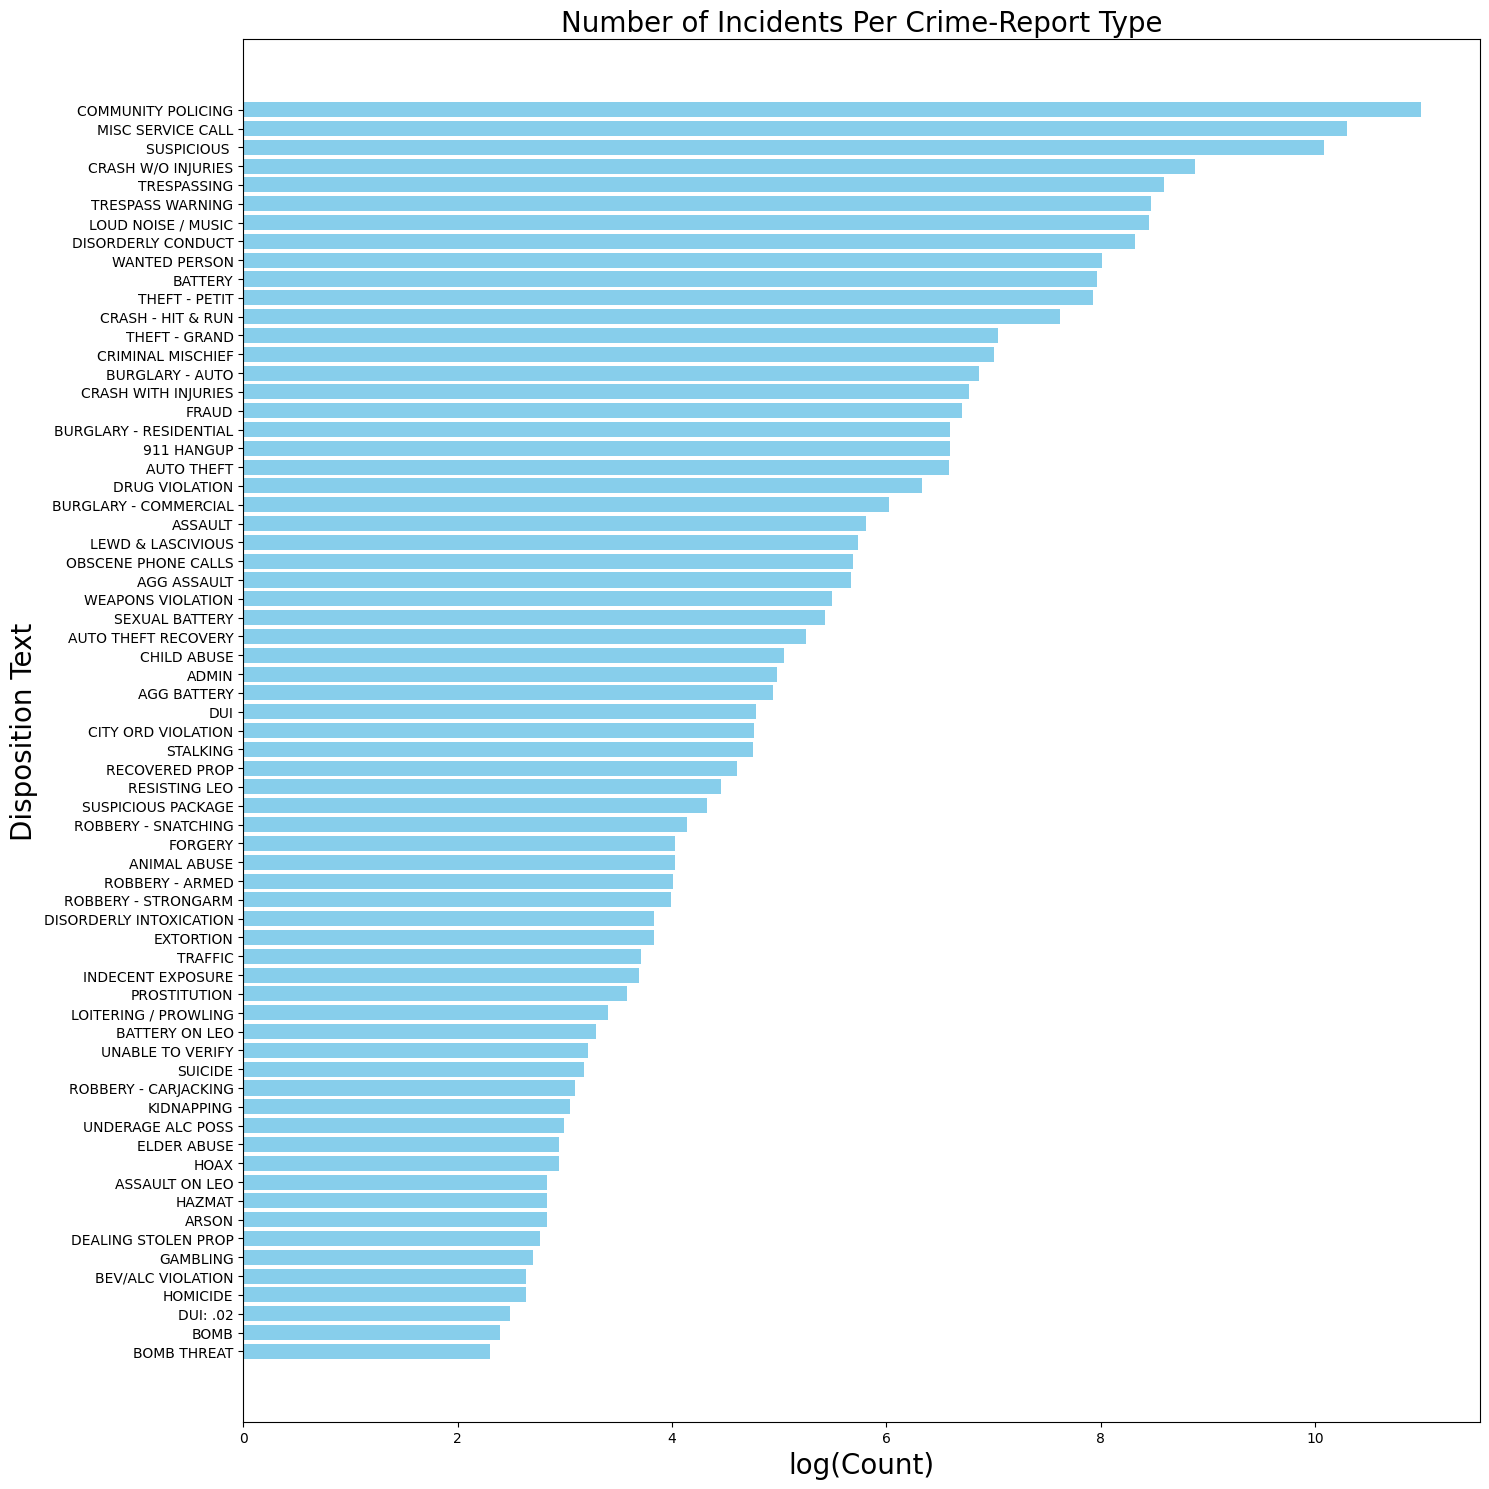
\includegraphics[width=0.8\textwidth]{Figures/Number of Incidents Per Crime-Report Type.png}
    \caption{Number of Incidents Per Crime-Report Type}
    \label{fig:crime-report}
\end{figure}

\subsection{Temporal Analysis}

Temporal data analysis revealed trends over different timescales, including monthly, daily, and hourly crime rates. Peak crime hours and seasonal variations were identified. The hourly distribution of crime reports is shown in Figure \ref{fig:crime-hour}.

\begin{figure}[!htbp]
    \centering
    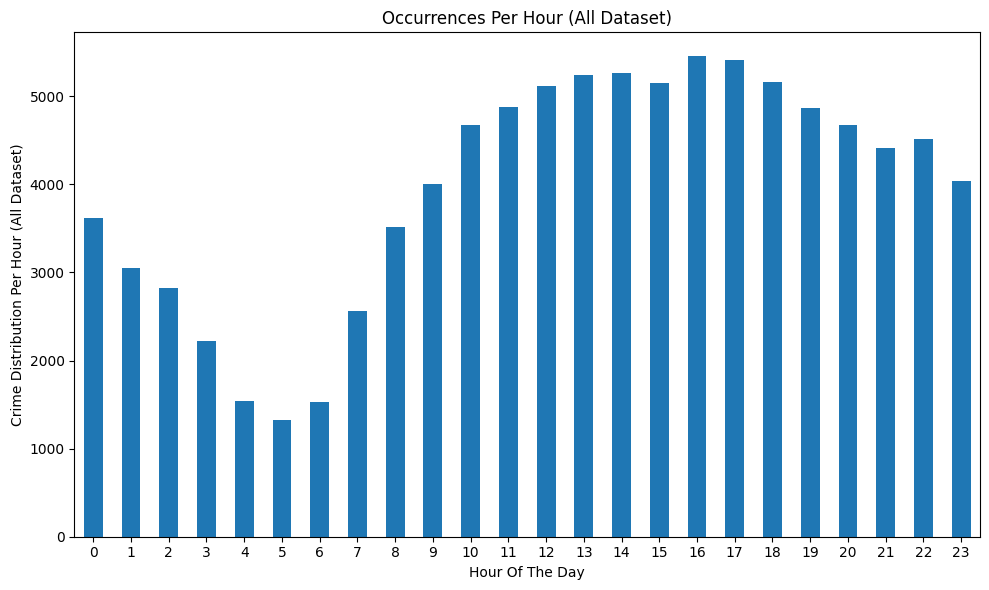
\includegraphics[width=0.8\textwidth]{Figures/Crime Distribution Per Hour (All Dataset).png}
    \caption{Crime Distribution Per Hour -- All 2023}
    \label{fig:crime-hour}
\end{figure}

\section{Crime Heatmap Generation}

The core of our project involved training a Conditional GAN (pix2pix) to take geographic maps as input and generate corresponding crime heatmaps. The overview of the pix2pix model is shown in Figure \ref{fig:pix2pix}. The model was trained on a dataset of geographical maps and corresponding crime heatmaps. The trained model was then used to generate crime heatmaps. Figure \ref{fig:heatmap} shows an example of a generated crime heatmap. To assess the model's performance, we compared the generated heatmaps with the actual heatmap by calculating the Mean Squared Error (MSE) between the two. As a baseline, we also calculated the MSE between the actual heatmap and a heatmap generated by randomly assigning crime reports to locations. Table \ref{tab:mse} shows the MSE values for the actual heatmap, the random heatmap, and the generated heatmap. The lower MSE value for the generated heatmap compared to the random heatmap indicates that the pix2pix model is able to generate more accurate crime heatmaps.

\begin{table}[!htbp]
    \centering
    \begin{tabular}{|c|c|}
        \hline
        \textbf{Heatmap Type} & \textbf{MSE}       \\
        \hline
        Random Heatmap        & 3.9543179869651794 \\
        pix2pix               & 0.9491354823112488 \\
        \hline
    \end{tabular}
    \caption{Mean Squared Error (MSE) for Heatmaps}
    \label{tab:mse}
\end{table}

\begin{figure}[!htbp]
    \centering
    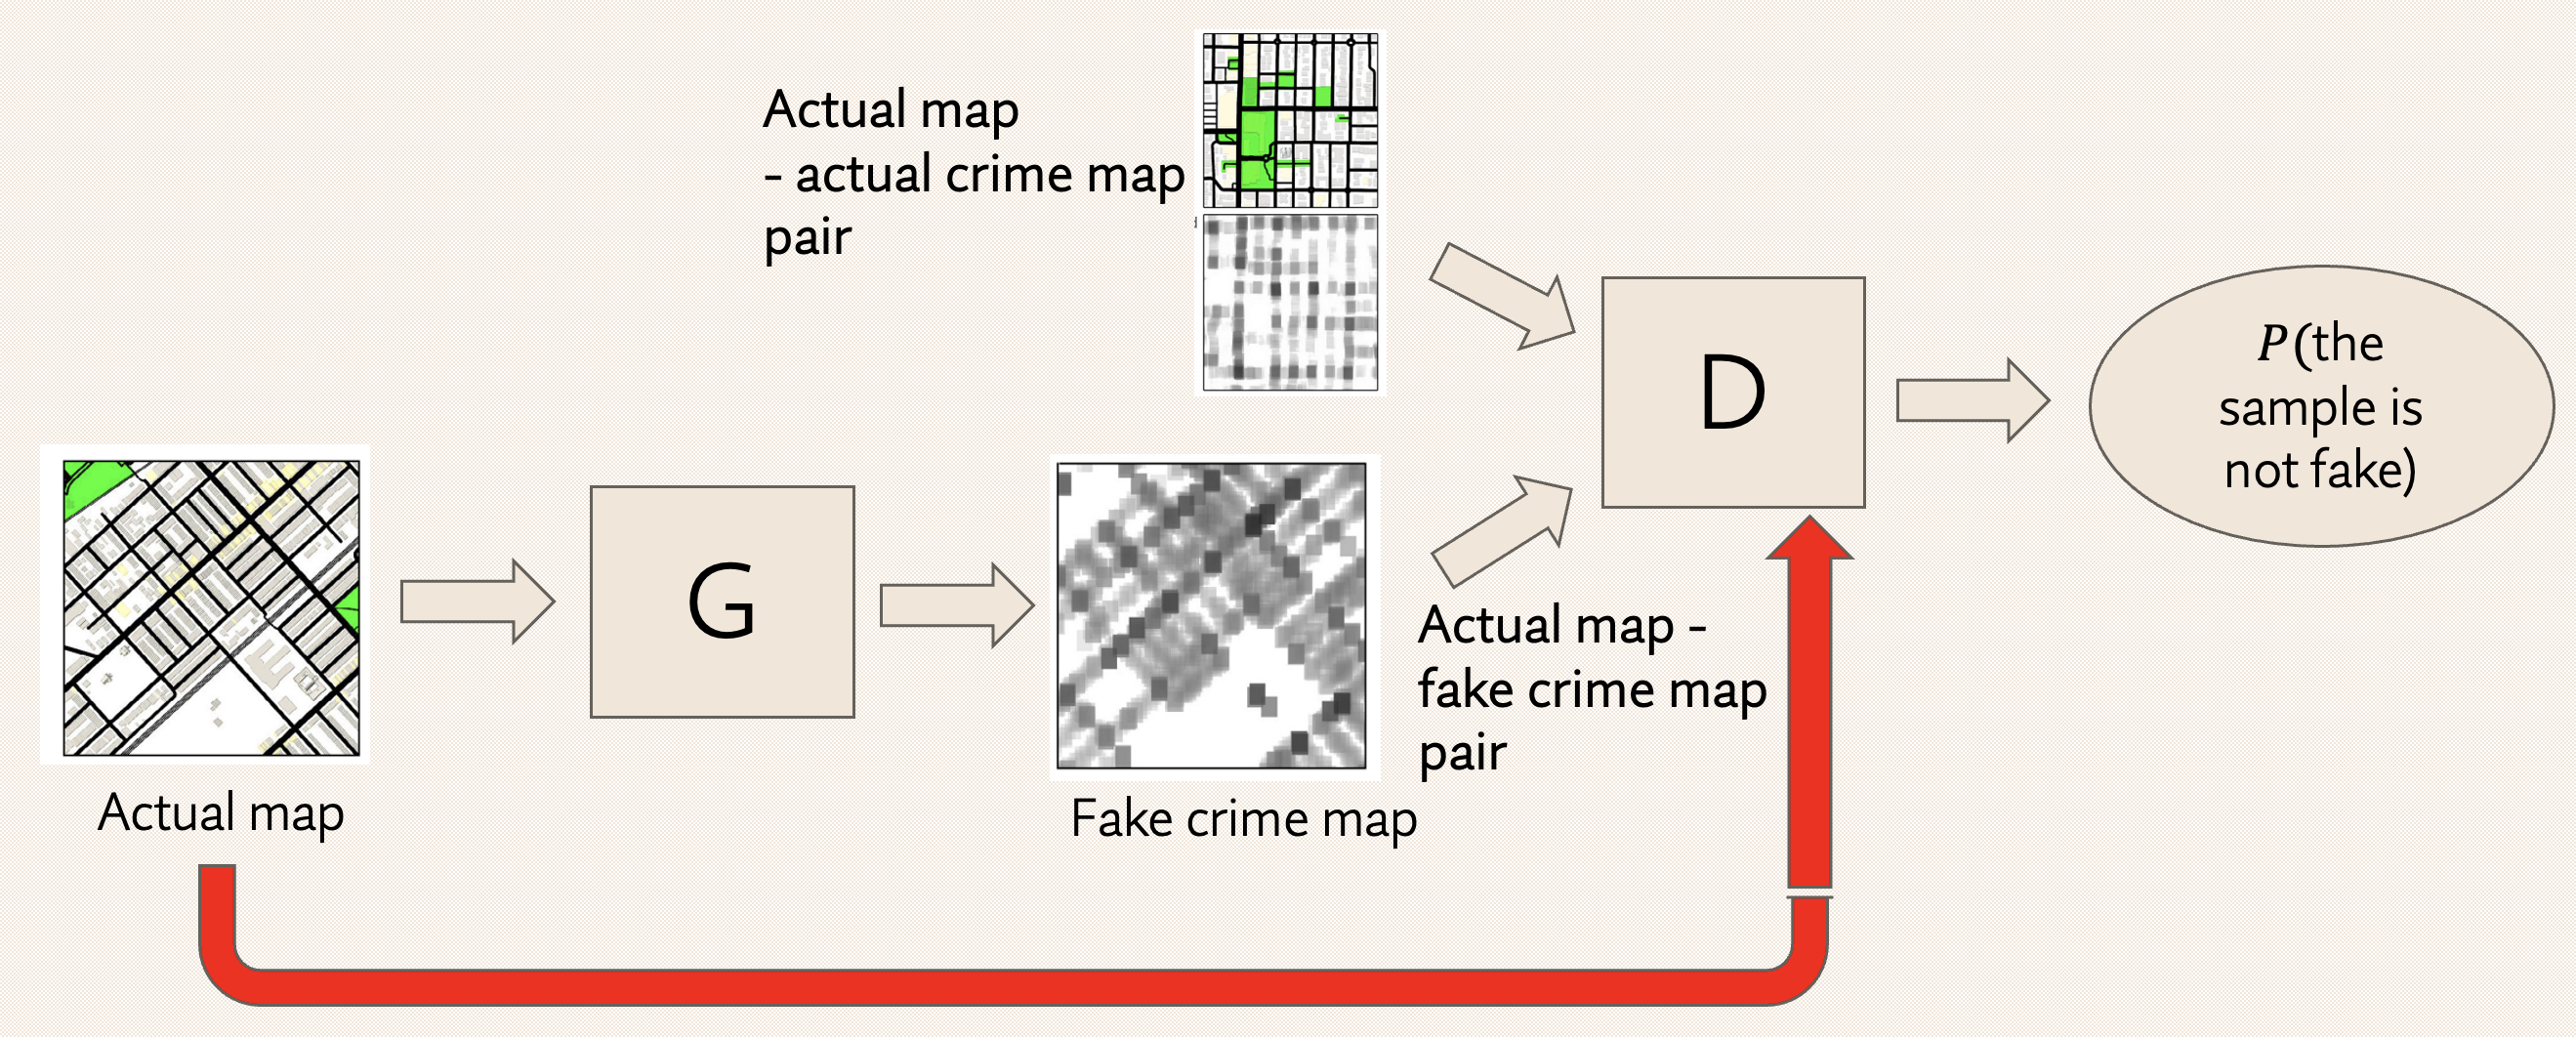
\includegraphics[width=1\textwidth]{Figures/conditionalgan.png}
    \caption{Pix2pix Model Diagram}
    \label{fig:pix2pix}
\end{figure}

\begin{figure}[!htbp]
    \centering
    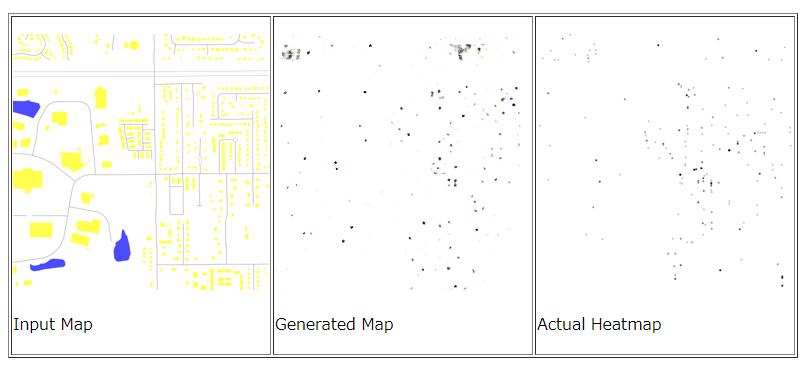
\includegraphics[width=0.8\textwidth]{Figures/Generated heats.png}
    \caption{Generated Crime Heatmap}
    \label{fig:heatmap}
\end{figure}

\section{Conclusion}

Our project demonstrated the potential of using advanced machine learning techniques like GANs for urban planning and public safety applications. Future work will focus on improving model accuracy, developing a user-friendly interface for creating hypothetical scenarios, and deploying a web application for broader accessibility.

\end{document}